\section{Design Space Exploration on EBeSS}	\label{sec:exp}
%
EBeSS is an energy-aware simulator supporting peripheral and energy managing strategy configurations for self-powered system.
With EBeSS, developers can optimize the hardware parameters of self-powered system (such as the capacitor size), and select appropriate energy managing strategy to achieve the maximum task completion performance. 
This section explores the design space of capacitor and energy managing strategy selection under different power traces and different peripheral numbers.

\subsection{Capacitor Design Space Considering Peripherals}
%
In this part, we explore the capacitor design space for self-powered system with different number of peripherals. 
Based on the \emph{brgMonitor} application, we scale the peripheral number in the application from zero to five, and simulate the completed task number within 10 minutes.
Figure~\ref{fig:CapVsBenchmark} shows the design space of capacitor size in self-powered system.
% Explainations.
From the figure, we observe a design edge for a self-powered system with different occupancy of peripherals to optimize the task completion rate.

\begin{figure}[!htpb]
	\centering
	\vspace{-5pt}
	\includegraphics[width=0.4\textwidth]{}
	\vspace{-5pt}
	\caption{The task completion curve of system using multiple peripherals and different capacitor sizes.}	\label{fig:CapVsBenchmark}
\end{figure}

\subsection{Explore Energy Managing Strategy Selection}
%
With an optimal hardware platform, this part explores the energy managing strategy selection with different energy supply conditions.
We scans the combination of different power traces and capacitors, and explores the suitability of different energy managing strategies.

Three popular existing energy managing strategies in the energy harvesting system are analyzed, that is, backup-restore~\cite{Ma2015Architecture}, state-retention~\cite{wang2017a130nm}, and DVFS~\cite{fletcher2017powerDVFS}.
\begin{itemize}

\item \textbf{State-retention}\\ 
State retention is a conventional energy managing strategy that all the peripherals enter an ultra-low cost sleep mode when the power supply is not enough.
During the sleeping stage, the system suffers a leakage power consumption to realize hardware states retention in the volatile memories.

\item \textbf{DVFS}\\ 
DVFS is an energy managing strategy used to dynamically adjust the system performance according to energy supply condition.
DVFS enables the system to execute at lower speed with lower energy consumption when the energy supply is limited, and execute at higher speed when the energy supply is sufficient.

\item \textbf{Backup-restore}\\ 
Backup-restore is a zero-leakage energy managing strategy that can bridge across power failure conditions by backing up and restoring the volatile execution states into nonvolatile memories. 
By moving the states into nonvolatile memory, the system can be safely shutdown to avoid leakage power during the outages and is most reliable in energy harvesting systems.

\end{itemize}

From the definition of the three energy managing strategies, it is obvious that, the performance of these strategies is affected by the system energy supply, which is determined the power trace and the system capacitor size.
Therefore, we explore the search space of the combination of power trace and capacitor size.

\begin{figure}[!htpb]
	\centering
	\vspace{-0pt}
	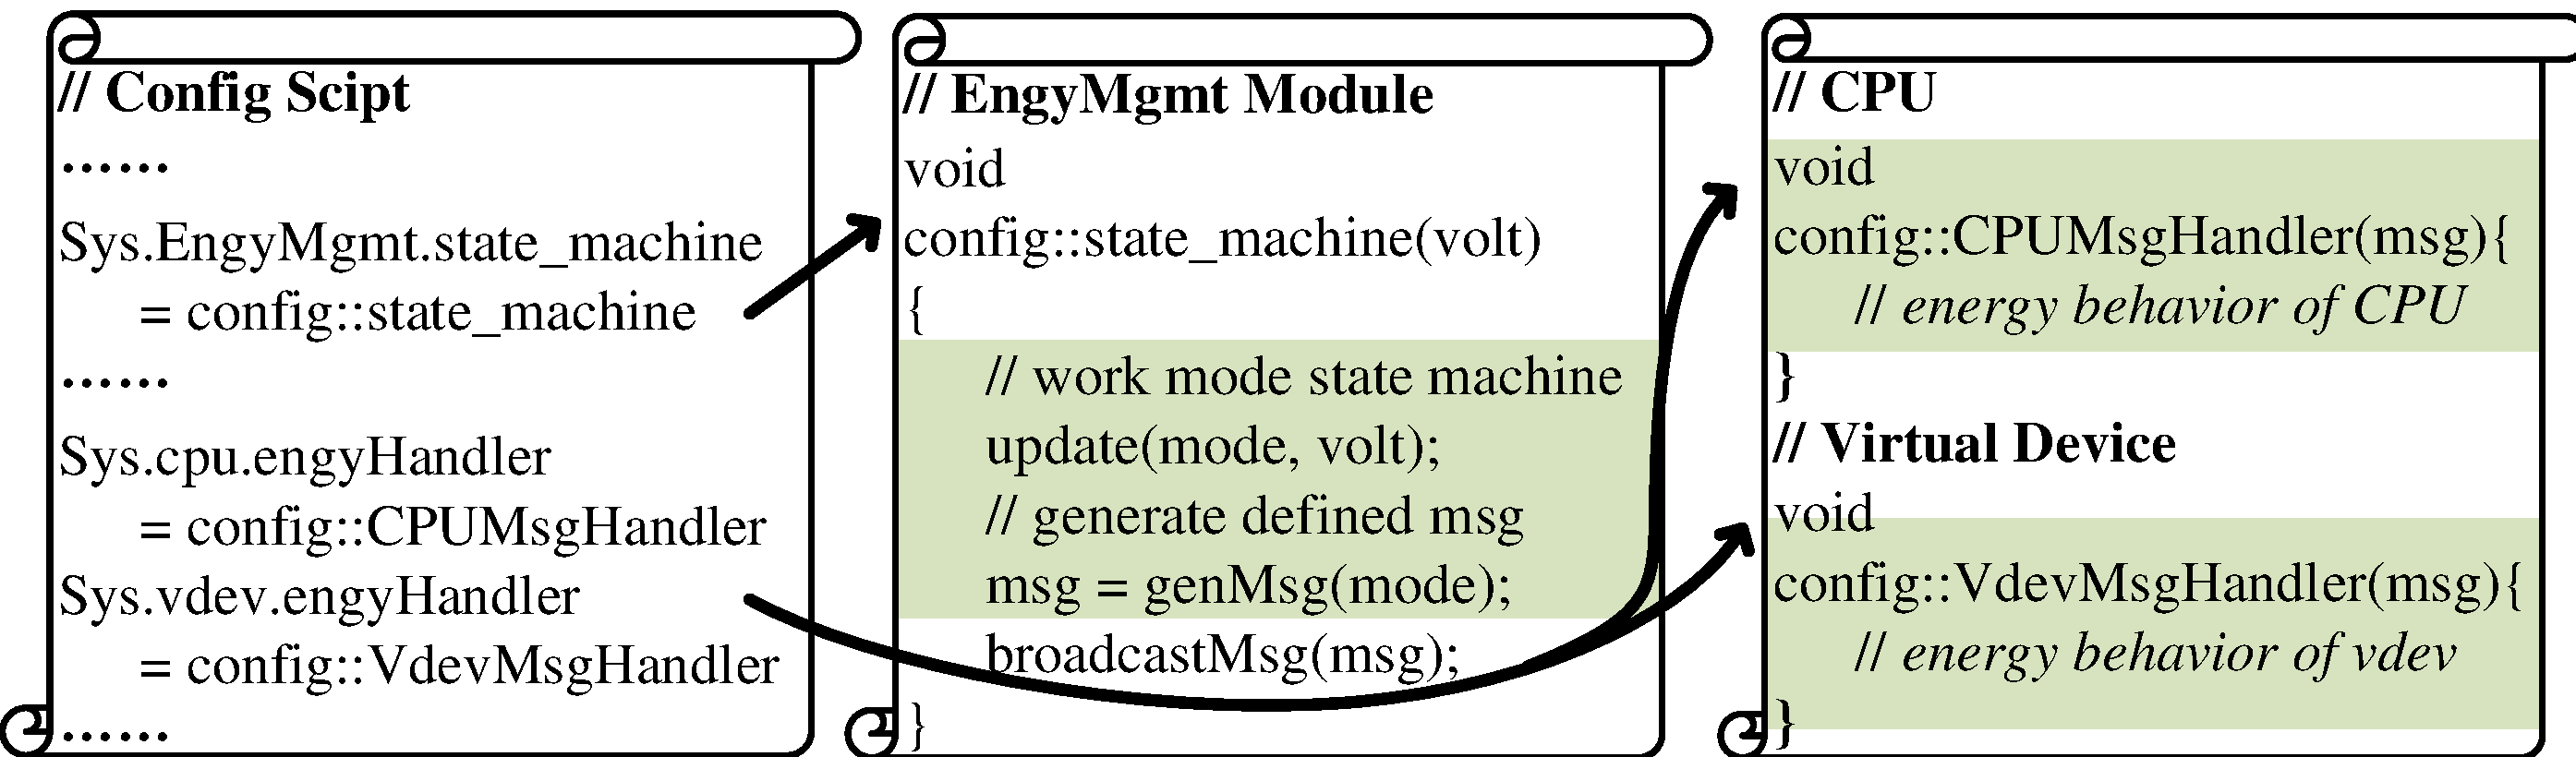
\includegraphics[width=0.5\textwidth]{EMStrategyConfig}
	\vspace{-15pt}
	\caption{The task completion curve of system using multiple peripherals and different capacitor sizes.}	\label{fig:EMStrategyConfig}
\end{figure}

We configure the energy managing strategy by editing the state machine in EMM to generate energy message, and the energy message handler in CPU and virtual device source code, as shown in Figure~\ref{fig:EMStrategyConfig}.
Figure~\ref{fig:HotpotGraph} (a-c) shows the performance hotpot graph when executing the \emph{brgMonitor} benchmark using each of these strategies.
% Explanations
Comparing the performance hotpot graph of these energy managing strategies, Figure~\ref{fig:HotpotGraph} (d) shows the distribution of the optimal energy managing strategy selection.
We can conclude that ...  

\begin{figure}[!htpb]
	\centering
	\vspace{-5pt}
	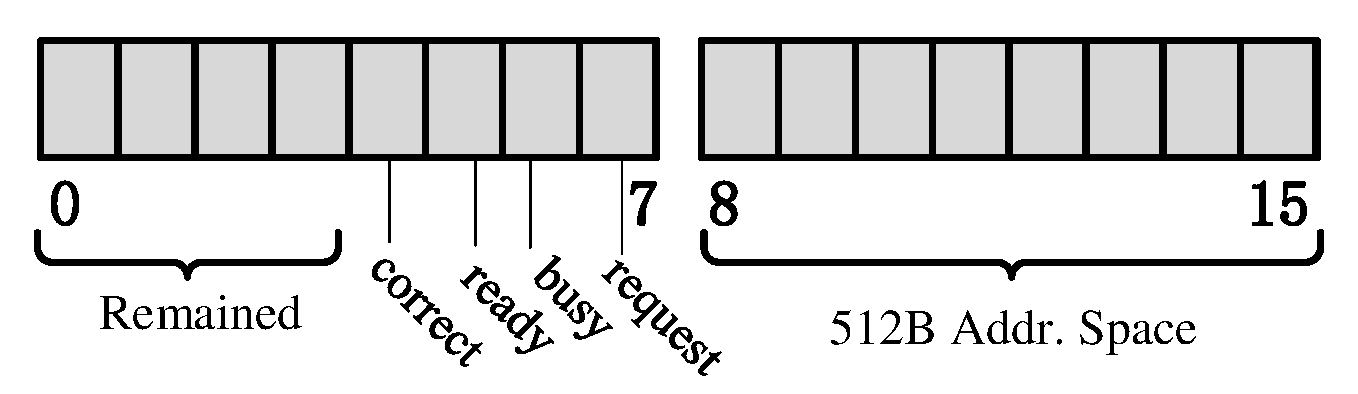
\includegraphics[width=0.4\textwidth]{VirtualDeviceAddress}
	\vspace{-5pt}
	\caption{The task completion curve of system using multiple peripherals and different capacitor sizes.}	\label{fig:HotpotGraph}
\end{figure}

\subsection{Exploration Conclusion}	\label{sec:exp-sum}
%
In conclusion, experiment explores the affect of the power supply density and the application types. 
Results show that, DVFS has the ability to take better usage of the too low and the too high energy supply.
On the other side, ModeCvrt and DVFS have the advantages in adjusting the energy usage of CPU and peripherals, respectively.
When the computing operations is dominating, DVFS has better performance to take fully usage of power supply.
When the I/O operations are dominating, ModeCvrt is the better choice to avoid the leakages of the idle peripherals.

\begin{comment}
\bibliographystyle{ACM-Reference-Format}
\bibliography{references} 
\end{comment}